\documentclass{article}
\usepackage{amsmath}
\usepackage{breqn}
\usepackage{color}
\usepackage{hyperref}
\usepackage{datetime}
\usepackage{graphicx}

\definecolor{heavyblue}{cmyk}{1,1,0,0.25}

\newcommand{\thetitle}{SEME 2016: OptionWay Project Report}
\newcommand{\theauthors}{Malcolm Roberts, Matteo Aletti, Athmane Bakhta, Boris Nectoux}

\title{\thetitle{}}
\author{\theauthors{}}

\hypersetup{
  pdftitle={\thetitle},
  pdfpagemode=UseOutlines,
  citebordercolor=0 0 1,
  colorlinks=true,
  allcolors=heavyblue,
  breaklinks=true,
  pdfauthor={\theauthors},
  pdfpagetransition=Dissolve,
  bookmarks=true
}

% Specify ISO date format:
\yyyymmdddate
\renewcommand{\dateseparator}{-}

\def\abs#1{{\left|#1\right|}}
\def\(#1\){{\left(#1\right)}}
\def\nobr#1{\hiderel{#1}}

\def\aow{\alpha_{\rm{OW}}}
\def\aobs{\alpha_{\rm{obs}}}
\def\anew{\alpha_{\rm{new}}}
\def\pmin{p_{\rm{min}}}


\begin{document}

\maketitle

\begin{abstract}
  We report on the \emph{Semaines d'Etude Maths-Entreprises} OptionWay
  (\url{https://www.optionway.com}) project.  OptionWay is an online
  travel agent which allows clients to buy flights for cheaper by
  taking into account the stochasticity of flight price over time.  In
  order help clients make useful decisions, they offer an estimate of
  how likely an asking price is likely to be realiastic.  The
  objectives for the workshop were to test this estimator, and, if
  time permits, to improve this estimator.  We show that the estimator
  is overly optimistic and show early work on developing an
  alternative.
\end{abstract}

\section{Introduction}

Travellers wishing to purchase a flight for a specific day to a
particular destination are faced with a problem: how can they find the
cheapest flight which matches their criteria?  Since the advent of
online travel agents, it is easy to find the cheapest price available
that day, and multiple services are available.  The travel agent
offers a variety of prices from multiple airlines, and the consumer is
free to choose whether or not they wish to buy.  At this point one
would think that the problem is solved, but one must remember that
there is another player in this particular economic game: the airline,
which seeks to sell seats on planes in order to maximize its own
profit.

In general, there are several airlines which compete on a particular
route, such as Paris--New York, and the airlines will vary their prices
according to their own individual strategies (strategies which, we add
parenthetically, produce seemingly bizarre prices).  The airlines
compete with each other, but they can also increase their profit by
adopting a strategy which increases the likelihood that an individual
consumer will purchase a ticket.  In addition, there are circumstances
where a consumer has very low price sensitivity, so it might be good
to occasionally offer higher prices in case such a client is looking
for a flight at the same moment when the high prices are in effect.

The effect of this on the consumer is that there is a significant
amount of variance in the price of the cheapest flight available.  If
the Paris--New York flight is \$1000 today, it might be \$900 next
week, or perhaps \$1100.  Thus the optimal strategy for the consumer
is to check the cost each day to determine the range of prices
available and then to use that information in order to try and get a
better price.  Each day the traveller will visit various websites,
collect data, and, when they think that they have enough information,
start looking for a flight.  While there may certainly be some
travellers who find this sort of activity a great way to spend a
Friday night, the vast majority will probably find the use of their
time sub-optimal for what may end up being a fairly minimal savings in
cost.

The online travel agent OptionWay (\url{https://www.optionway.com})
autmoates this process; the traveller specifies their destination and
travel dates, the price that they are willing to pay for the trip, and
the length of time that they want OptionWay to look for the ticket.
If their criteria are satisfied during this time, OptionWay
automatically buys the ticket when the specified price is available.
Using this method, the traveller is saved the drudgery of manually
searching for flights on a daily basis.

However, the demand price may or may not be likely to appear in the
specified search period.  For example, if the traveller wants to fly
Paris--New York for \$400, they are likley to never find a ticket at
such a price.  OptionWay would like to provide an estimate for the
probability of the chance of success of their demand.

\section{Data and Analysis}

OptionWay provided us with sample data for flights to various
destinations.  The data was composed of all the flight prices for a
particular route for travel on a variety of dates, with flight prices
available from 130 days before the flight to the day of.  Data was not
necessarily available for each day.  There were 12 routes available.
Data was given in the form of csv files, which ranged in size from 13M
to 2.3G.  We created a \texttt{python} script to read and analyze the
data, which is available at
\url{https://github.com/malcolmroberts/seme2016}.  Not all data files
were analyzed due to limited time and computational resources.  We
show a sample of such data in Figure~\ref{PARFCO_SAT_7_nonorm} for
flights between Paris and Rome from Saturday to Saturday.  In
Figure~\ref{PARRUN_SAT_7_nonorm}, we show data for Paris--Ile Réunion,
also for a Saturday-to-Saturday trip.  While both show a large amount
of variance, the Paris-Rome trip shows a stronger tendency for the
price to rise nearer the travel date than the Paris--Réunion trip.

\begin{figure}
  \begin{center}
    % ./plots.py -f data/PARFCO_SAT_7.csv -d PARFCO_SAT_7_nonorm
    % asy datagraphs -u "ymax=500"
    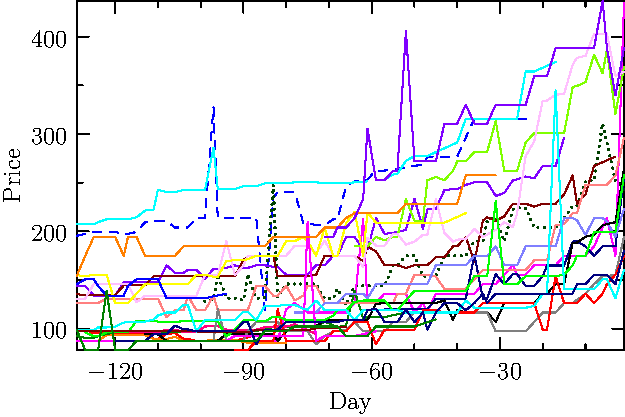
\includegraphics{pdf/PARFCO_SAT_7_nonorm}
    \label{PARFCO_SAT_7_nonorm}
    \caption{Minimum available price as a function of number of days
      before the lgiths for PAR--FCO from Saturday to Saturday for a
      variety of departure dates. Prices abore 500 were excluded.}
  \end{center}
\end{figure}

\begin{figure}
  \begin{center}
    %  ./plots.py -f data/PARRUN_SAT_7.csv -d PARRUN_SAT_7_nonorm
    % asy datagraphs -u "ymax=3000"
    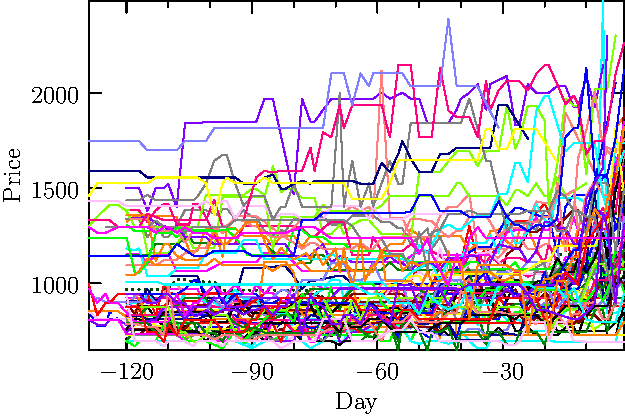
\includegraphics{pdf/PARRUN_SAT_7_nonorm}
    \label{PARRUN_SAT_7_nonorm}
    \caption{Minimum available price as a function of number of days
      before the lgiths for PAR--RUN from Saturday to Saturday for a
      variety of departure dates. Prices abore 3000 were excluded.}
  \end{center}
\end{figure}

\section{Probability Estimators}
The probability of an asking price $p_d$ being achieved during a
search interval $T$ is denoted by $\alpha$.  Let $p(t)$ denote the
minimum price at time $t$, in days, for the a given flight, and $t_0$
the time when the traveller starts looking for a ticket.

\subsection{OptionWay Estimator}
As a rough estimate, OptionWay uses the following formula to predict
the probability that the client will succeed:
\begin{dmath}
  \alpha_{\rm{OW}}(t_o,T,p_d)
  = \frac{1}{1 + \frac{4500 p(t_0)}{4.5 T}e^{-11 p_d / p(t_0)}}.
  \label{owalpha}
\end{dmath}
The motivation behind this formula was to construct a function that
gives a higher probability when $p_d$ and $T$ are large.

We can test the accuracy of equation~\eqref{owalpha} agains the given
data.  In Figure~\ref{PARRUN_SAT_7_a0}, we show the a colourmap of the
probability of successfully finding a flight at a price $p_d$ for
$t_0=30$.  Notably, there is a large increase in probability in about
30 days before travelling.  We can compare the obsered probability,
$\alpha_{\rm{obs}}$ against equation~\eqref{owalpha} for individual
lines.  Such a comparison is shown in Figure~\ref{PARRUN_SAT_7_a1_A0},
which shows $\alpha_{\rm{obs}}-\alpha_{\rm{OW}}$.  The difference is
almost entirely negative, indicating that the OptionWay estimate errs
heavily on the side of optimism.  
\begin{figure}
  \begin{center}
    %./test.py -f data/PARRUN_SAT_7.csv -a0
    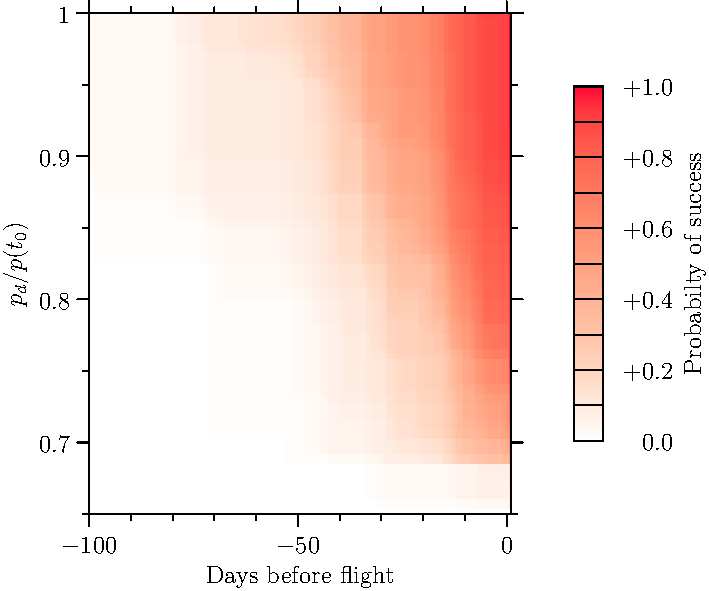
\includegraphics{pdf/PARRUN_SAT_7_a0}
    \label{PARRUN_SAT_7_a0}
    \caption{Probability of success $\alpha_{\rm{obs}}$ for an asking
      price $p_d$ for PAR--RUN for $t_0=30$.}
  \end{center}
\end{figure}
\begin{figure}
  \begin{center}
    %./test.py -f data/PARRUN_SAT_7.csv -a1 -A0
    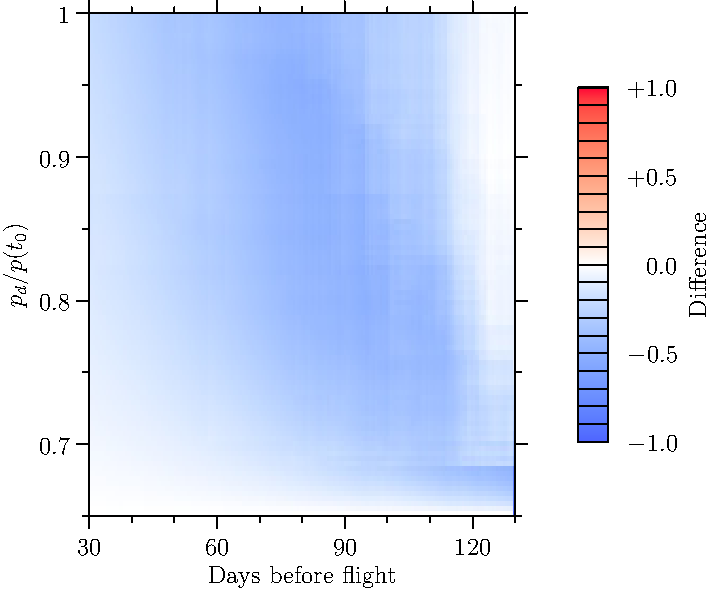
\includegraphics{pdf/PARRUN_SAT_7_a1_A0}
    \label{PARRUN_SAT_7_a1_A0}
    \caption{Difference $\alpha_{\rm{obs}} - \alpha_{\rm{OW}}$ in
      prediction of probability of success between empirical
      measurement and equation~\eqref{owalpha} for an asking price
      $p_d$ for PAR--RUN for $t_0=30$.}
  \end{center}
\end{figure}

In Figure~\ref{plotA0} we show the $L_1$ diference between $\aobs$ and
$\aow$ as a function of $t_0$ for a variety of flights.  For a
majority of the flights considered, $\aow$ has poor accuracy for early
$t_0$, but this improves as the departure date approaches; near the
date of departure, $\aow$ succesfully predicts that a deal is highly
unlikely.  However, there are three cases for which $\aow$ performs
much better.  What is the difference?  Is there some property of these
flights which explains this difference?
\begin{figure}
  \begin{center}
    % ./rundiffA0.sh
    % diff0/PARFCO_MON_123/normvst0.dat,diff0/PARMAD_SAT_7/normvst0.dat,diff0/PARFCO_MON_45/normvst0.dat,diff0/PARNYC_SAT_7/normvst0.dat,diff0/PARFCO_SAT_7/normvst0.dat,diff0/PARRUN_ALL/normvst0.dat,diff0/PARMAD_MON_123/normvst0.dat,diff0/PARRUN_SAT_7/normvst0.dat,diff0/PARMAD_MON_45/normvst0.dat
    %asy datagraphs -u"dolegend=true" -u"legendlist=\"PARFCO_MON_123,PARMAD_SAT_7,PARFCO_MON_45,PARNYC_SAT_7,PARFCO_SAT_7,PARRUN_ALL,PARMAD_MON_123,PARRUN_SAT_7,PARMAD_MON_45\""
    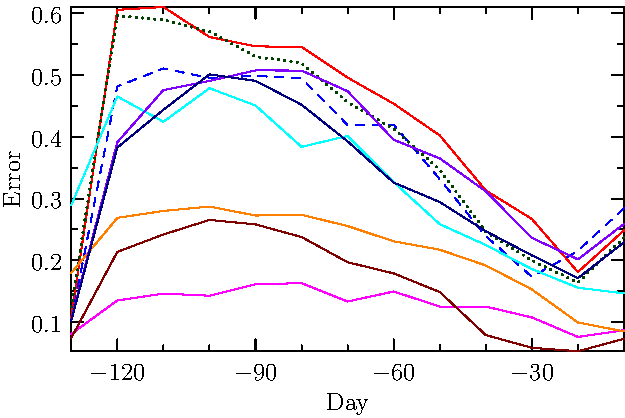
\includegraphics{pdf/plotA0}
    \label{plotA0}
    \caption{Difference between $\alpha_{\rm{OW}}$ and
      $\alpha_{\rm{obs}}$ as a function of $t_0$.}
  \end{center}
\end{figure}

In equation~\eqref{owalpha}, the asking price $p_d$ is divided by the
current minimum price $p(t_0)$.  We can also re-create
figures~\ref{PARFCO_SAT_7_nonorm} and~\ref{PARRUN_SAT_7_nonorm} with
the results scaled by $p(t_0)$.  The results are shown in
Figures~\ref{PARFCO_SAT_7_norm} and~\ref{PARRUN_SAT_7_norm}.  After
normalizing the data, the difference is much more clear; in
Figures~\ref{PARFCO_SAT_7_norm}, there is a strong ris in prices at
around $t_0=-30$, which is much less pronounced in
Figure~\ref{PARRUN_SAT_7_norm}.  The formula given for $\aow$ is
designed to deal with the variance in prices, but neglects any trend.
\begin{figure}
  \begin{center}
    % ./plots.py -f data/PARFCO_SAT_7.csv -d PARFCO_SAT_7_norm -npt0
    % asy datagraphs -u "ymax=2"
    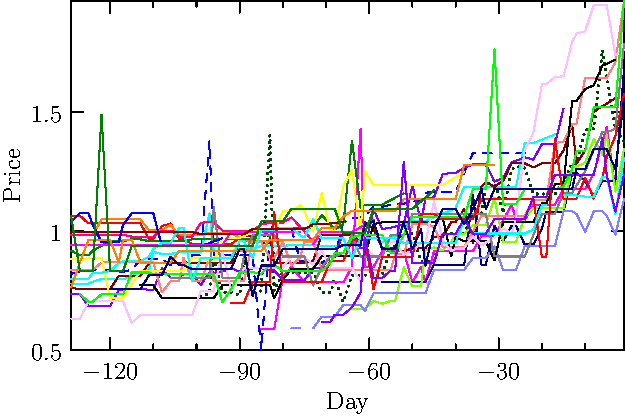
\includegraphics{pdf/PARFCO_SAT_7_norm}
    \label{PARFCO_SAT_7_norm}
    \caption{Minimum available price, normalized by $p(t_0)$, as a
      function of number of days before the lgiths for PAR--FCO from
      Saturday to Saturday for a variety of departure dates. Prices
      with $p_d/p(t_0) > 2$ were excluded.}
  \end{center}
\end{figure}

\begin{figure}
  \begin{center}
    %./plots.py -f data/PARRUN_SAT_7.csv -d PARRUN_SAT_7_norm  -npt0
    % asy datagraphs -u "ymax=2"
    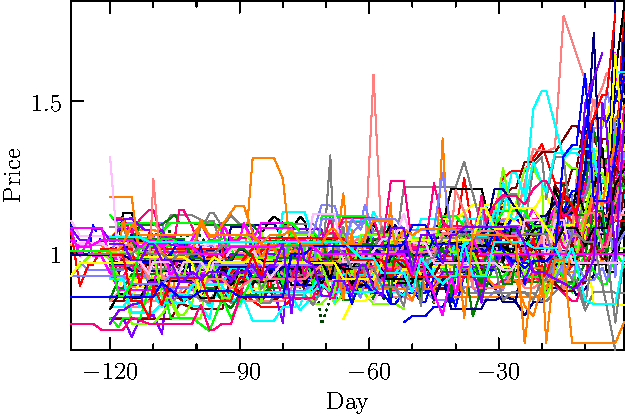
\includegraphics{pdf/PARRUN_SAT_7_norm}
    \label{PARRUN_SAT_7_norm}
    \caption{Minimum available price, normalized by $p(t_0)$, as a
      function of number of days before the lgiths for PAR--RUN from
      Saturday to Saturday for a variety of departure dates.  Prices
      with $p_d/p(t_0) > 2$ were excluded.}
  \end{center}
\end{figure}


\subsection{Alternative Estimators}

OptionWay's predictor given in equation~\eqref{owalpha} has several
parameters, and an obvious possibilty for improving the accuracy of
the prediction is to fit these parameters to the data.  We computed
the $L_2$ error and tried to find the optimal parameters for each
route and $t_0$ using the Broyden–Fletcher–Goldfarb–Shanno (BFGS)
algorithm.  The advantage of this technique is that one can find
optimal parameter values for each individual case, which will, in
general, give much a much better prediction.  The method is
computationally expensive, and during the workshop we were able to
calculate a handful of cases.  When calibrated with 50 flights, the
$l_2$ error was reduced by approximately two orders of magnitude,
which is a significant improvement.  Given more time, it would be
interesting to continue this study.

We also looked at an alternative form for $\alpha$ based upon ad-hoc
reasoning for how the likelihood of finding a flight should behave.
The formula is givne in equation~\eqref{anew}, where $\pmin$ is the
global minimum price for the route, $a=8$, $b=12$, $c=7$, $d=7$,
$e=0.01$, and $S_0=10$ are adjustable paramters, $T_f$ is the time
remaining before the flight, and the score $S$ is given in
equation~\eqref{S}.  The motivation behind equation~\eqref{anew} is
that we penalize unlikely or impossible outcomes based, treat the
price as having constant mean and variance, and use more information
(and tunable parameters) in order to better match the data.
\begin{dmath}
  \label{anew}
  \anew = \frac{1}{
    1
    + \exp{\(S_0-S\)}
    + \frac{d}{T+10^{-6}}
    + e\frac{\pmin}{\max{\( p(t_0) - \pmin, 10^{-14}\)}}}
\end{dmath}
\begin{dmath}
  \label{S}
  S = a \frac{p_d}{p(t_0)} + b \(1 - \frac{\pmin}{p(t_0)}\) + c \frac{T}{T_f}
\end{dmath}
The $\frac{1}{T+10^{-6}}$ term penalizes those who are impatient, and
the $\frac{\pmin}{\max{\( p(t_0) - \pmin, 10^{-6}\)}}$ penalizes those
who are asking for a price below what is historically possible.  The
$\exp{\(S_0-S\)}$ term penalizes asking prices which are too cheap,
and also reinforces some of the same properties as found in the other
terms.  As can be seen in Figure~\ref{plotA1}, equation~\eqref{anew}
gives a much smaller prediction error than equation~\eqref{owalpha}.
However, the error does tend to inrease when the departure date and
$t_0$ are close; this can be explained by the fact that
equation~\eqref{anew} was designed based upon a simplified model where
the mean price does not change with time.  For certain groups of
flights, this is clearly not the case.  However, the new method does
provide a more accurate prediction.  The fact that it has more tunable
paraemters allows it to be tuned to a particular problem, though there
is the risk that one can over-tune the model.
\begin{figure}
  \begin{center}
    % ./rundiffA1.sh
    % diff1/PARFCO_MON_123/normvst0.dat,diff1/PARMAD_SAT_7/normvst0.dat,diff1/PARFCO_MON_45/normvst0.dat,diff1/PARNYC_SAT_7/normvst0.dat,diff1/PARFCO_SAT_7/normvst0.dat,diff1/PARRUN_ALL/normvst0.dat,diff1/PARMAD_MON_123/normvst0.dat,diff1/PARRUN_SAT_7/normvst0.dat,diff1/PARMAD_MON_45/normvst0.dat
    %asy datagraphs -u"dolegend=false" -u"legendlist=\"PARFCO_MON_123,PARMAD_SAT_7,PARFCO_MON_45,PARNYC_SAT_7,PARFCO_SAT_7,PARRUN_ALL,PARMAD_MON_123,PARRUN_SAT_7,PARMAD_MON_45\""
    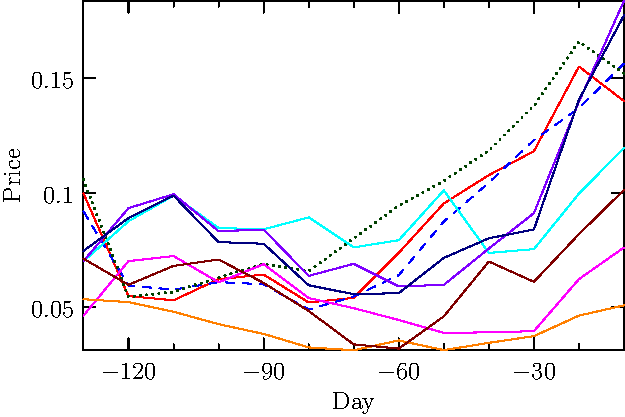
\includegraphics{pdf/plotA1}
    \label{plotA1}
    \caption{Difference between $\anew$ and $\alpha_{\rm{obs}}$ as a
      function of $t_0$.}
  \end{center}
\end{figure}

\section{Conclusion}

During the Semaines d'Etude Maths-Entreprises, OptionWay presented us
with the problematic of creating a test to determine the accuracy of
their probability estimator which is used to determing whether an
asking price for a certain flight will be available during a given
search window.  They provided us with a several data sets which we
used to test this hypothesis, and we were able to show that their
estimate was much too optimistic in the vast majority of cases.  In
addition, we were able to perform some initial work on determining
optimal parameters for their estimator, and also proposed an
alternative estimator.  Our alternative estimator has more parameters,
and has better precision, but requires more knowledge of the price
history.

Both our estimator and OptionWay's estimator have hand-selected
parameters.  In the time allotted, we were able to numerically
optimise the parameters for OptionWay's estimator certain cases, and
it would be interesting to continue this process for both OptionWay's
estimator and our new proposed estimator.  However, both estimators
had different performance based upon the behaviour of prices on the
particular route, which can be grouped into roughtly two types; one,
where the average price is constant, and one where there is an
increase in price starting about 40 days before departure.  This
indicates that a clustering analysis could be of use to determine
which type of behaviour is present, and then have design a model for
each cluster, giving a balance between precision and generality of the
model.  Finally, the problem faced by OptionWay is closely related to
well-studied problems in financial mathematics, and attack via a
statistical techniques is likely to give the best results.  We
understand that OptionWay is in the process of developing such a model
with an INRIA research group, and it will be interesting to see what level
of precision can be achieved.

\renewcommand{\abstractname}{Acknowledgements}
\begin{abstract}
  We would like to think that Semaines d'Etude Maths-Entreprises
  organizers, Didier Auroux, Cédric Boulbe, and Laurent Busé for their
  excellent work organizing this workshop.  We would also like to
  thank OptionWay (\url{https://www.optionway.com}), and in particular
  Nicolas Helin, Billy Girboux, and FIXME, for their help and
  participation during the workshop.
\end{abstract}

\end{document}
